\chapter{Theory}
\label{chap:theory}


% intro to the section
Energy dispersive X-ray spectroscopy (EDS) is a technique for analyzing the elemental composition of a sample with a spatial resolution, used in SEM and TEM.
The technique is based on excitation of core shell electrons, which are bound to the atom with different strengths in different elements, and thus the electron relaxation results in very specific photon energies.
EDS can be used to determine both the qualitative and quantitative composition of a sample.
This chapter will cover the theoretical formation of characteristic X-rays, the empirical adjustments done due to creation and detection issues, explain quantitative calculations, cover the parameters of a quality control program, and briefly explain the basics of a SEM.










\section{Theoretical view on characteristic X-rays}
\label{sec:theory:theoreticalxray}


This section is primarily based on Hollas \cite[Ch. 8.2]{hollas_modern_2004} and Goldstein \cite[Ch. 4.2]{goldstein_scanning_2018}.
It covers the theoretical physics behind creation of characteristic X-rays.










\subsection{Formation of characteristic X-rays}
\label{sec:theory:theoreticalxray:formation}
The formation of characteristic X-rays is an inelastic quantum mechanical scattering process in two steps.
In the following four equations the subscripts are referring to specific electrons in order to distinguish between them, which is also used in \cref{fig:theory:theoreticalxray:formation}
The figure shows the formation of characteristic X-rays with the atom as in the Bohr model, where ionization and relaxation is divided into two steps.
The three relaxations showed produce three characteristic X-rays with different energies.
The naming of the X-rays are covered in \cref{sec:theory:theoreticalxray:naming}, and illustrated in \cref{fig:theory:theoreticalxray:naming:lines}.
Only the relevant electrons are shown in the figure.
In the ionization step, the electron from the beam ionize the atom which ejects an electron from the core orbital.
In the relaxation step an electron from a higher orbital relaxes to the hole left by the ejected electron, and the figure shows the three possible relaxations.
The first step is described in \cref{eq:theory:theoreticalxray:formation:step1}, where electron e$^-_{1}$ from the incident electron beam eject electron $\textnormal{e}^-_{2}$ from the core orbital of atom A \cite[Eq. (8.12)]{hollas_modern_2004}.



% ionize the atom
\begin{equation}
    \label{eq:theory:theoreticalxray:formation:step1}
    \textnormal{e}^-_{1 \textnormal{, incident}} + A \rightarrow \textnormal{e}^-_{1 \textnormal{, outgoing}} + A^+ + \textnormal{e}^-_{2 \textnormal{, ejected}}
\end{equation}


% figures/formation_of_xrays_bohr.png
\begin{figure}[htb]
    \centering
    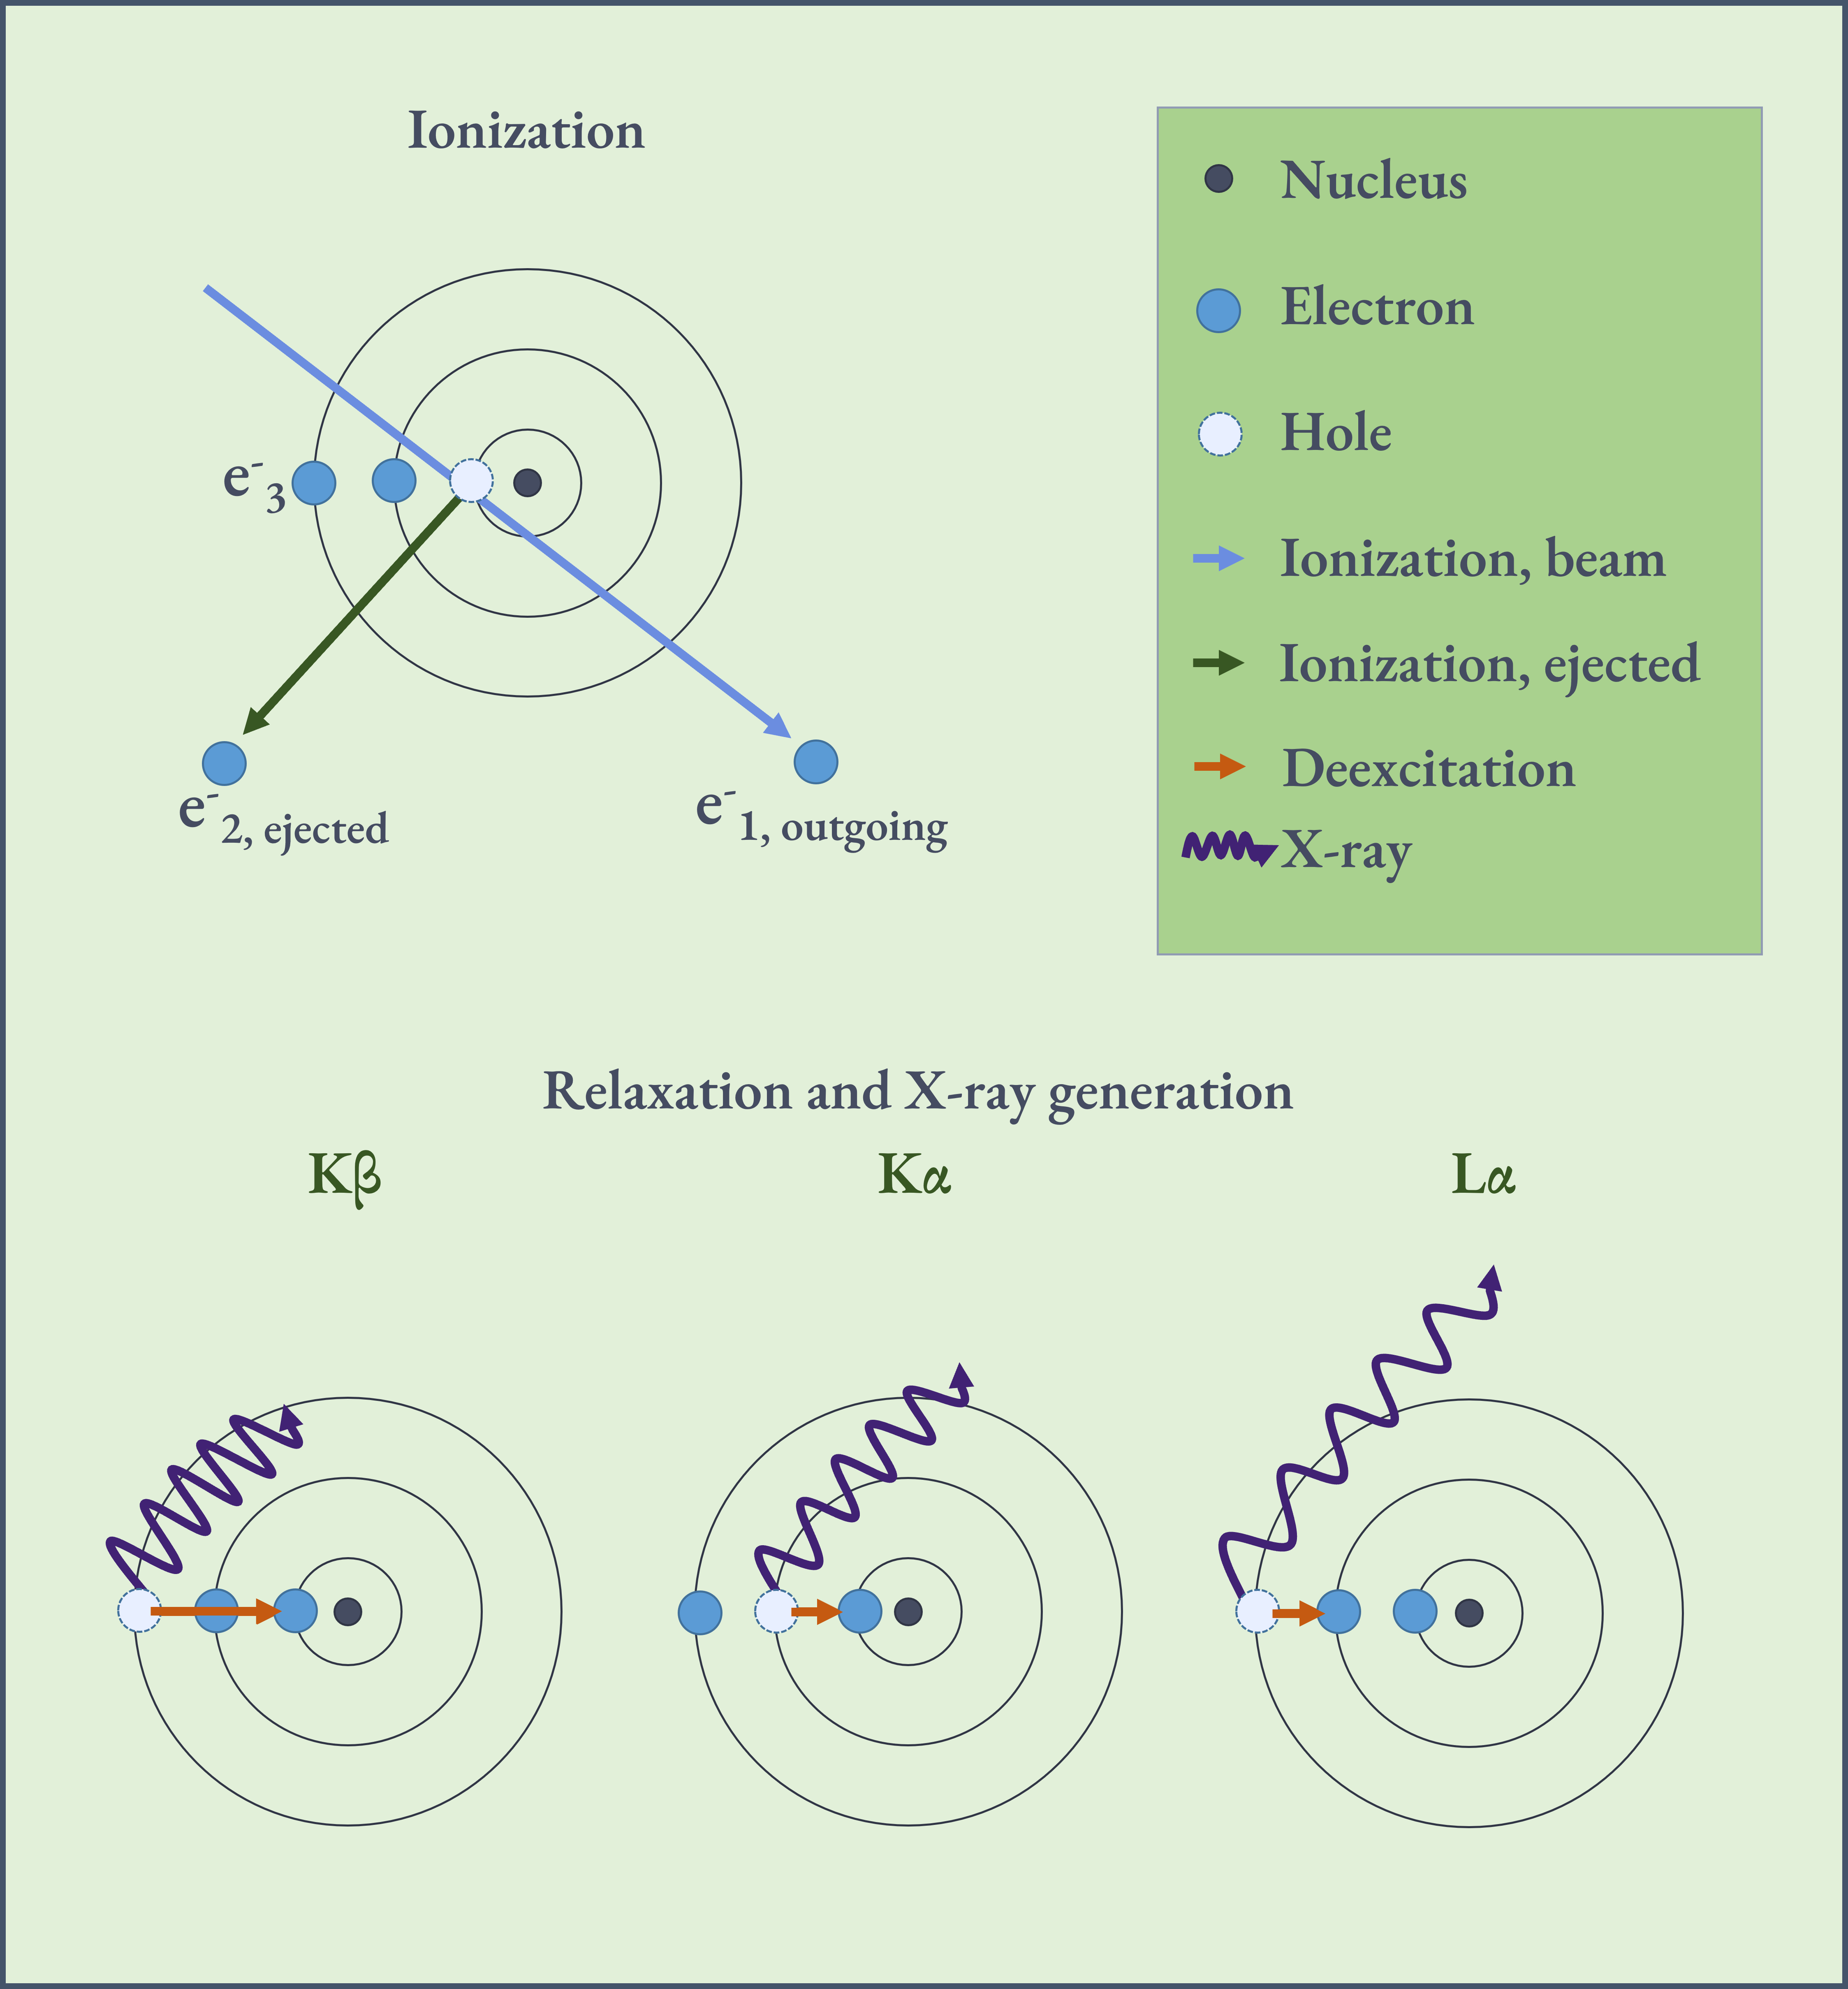
\includegraphics[width=0.85\linewidth]{figures/formation_of_xrays_bohr.png}
    \caption{
        The formation of characteristic X-rays with the atom as in the Bohr model, where ionization and relaxation is divided into two steps.
        The three relaxations showed produce three characteristic X-rays with different energies.
        Increased energy is illustrated as X-rays with shorter wavelengths.
    }
    \label{fig:theory:theoreticalxray:formation}
\end{figure}


% the energy of ionization, Goldstein eq 4.1
The incident electron from the beam loose energy to both breaking the binding energy of the core orbital and to the kinetic energy of the ejected electron.
The energy is given by \cref{eq:theory:theoreticalxray:formation:step1:energy}, and illustrated as the difference in energy level between the orbitals in \cref{fig:theory:theoreticalxray:naming:lines}.
The user can control the incident electron energy $E_{1 {\textnormal{, incident}}}$ by the acceleration voltage $V_{\textnormal{acc}}$ of the electron gun (and the current $I_{\textnormal{beam}}$ of the electron beam).
The energy of the characteristic X-ray is dependent on the binding energy of the core orbital, $E_{2 {\textnormal{, core shell, binding}}}$.
In EDS $E_{1 {\textnormal{, outgoing}}}$ and $E_{2 {\textnormal{, kinetic}}}$ serve no purpose \cite[Eq. (4.1)]{goldstein_scanning_2018}.

\begin{equation}
    \label{eq:theory:theoreticalxray:formation:step1:energy}
    E_{1 {\textnormal{, incident}}} = E_{1 {\textnormal{, outgoing}}} + E_{2 {\textnormal{, core shell, binding}}} + E_{2 {\textnormal{, kinetic}}}
\end{equation}

% relax the electron
In the second step electron $\textnormal{e}^-_{3}$ from a higher energy orbital relaxes to the hole in the core orbital of atom A, and the difference in energy is emitted as a photon with a specific energy $h\nu$ called the characteristic X-ray \cite[Eq. (8.12)]{hollas_modern_2004}.

% outer orbital relaxation
\begin{equation}
    \label{eq:theory:theoreticalxray:formation:step2}
    \textnormal{e}^-_{3 {\textnormal{, outer shell}}} \rightarrow \textnormal{e}^-_{3 {\textnormal{, inner shell}}} + h\nu_{\textnormal{X-ray}}
\end{equation}

The energy of the characteristic X-ray is the difference in energy between the ionized orbital and the orbital filling the hole, shown in \cref{eq:theory:theoreticalxray:formation:step2:energy}.
The equation specifies the energy of the X-ray as $h\nu$, but \cref{sec:theory:empirical} explains why users of EDS just use the energy directly, usually measured in eV or keV \cite[Eq. (4.2b)]{goldstein_scanning_2018}.

% the energy of the relaxation
\begin{equation}
    \label{eq:theory:theoreticalxray:formation:step2:energy}
    h\nu_{\textnormal{X-ray}} = E_{2 {\textnormal{, core shell, binding}}} - E_{3 {\textnormal{, outer shell, binding}}}
\end{equation}


% mention Auger electrons, because of the fluorescent (quantum) yield
% the kinetic energy is essential for Auger electrons, i.e. E_{2_{\textnormal{kinetic}}}
In the second step in \cref{eq:theory:theoreticalxray:formation:step2} it is also a probability that the relaxation energy is used to eject and give kinetic energy to another electron from a higher energy orbital.
This process results in two ejected electrons, both the ionized electron from the core orbital and a second ejected electron from a higher energy orbital.
The second ejected electron is called an Auger electron.
Auger electrons are used for surface studies, because they can penetrate around 2 nm solid material and thus does not escape from inside the sample.
The X-rays are emitted in all directions and penetrate typically 4000 nm, and are the signal in EDS.
The ratio between the characteristic X-ray photons and Auger electrons are known as the fluorescent (quantum) yield, $\omega$. %or sometimes $\Phi_F$.

% fluorescent yield, definition
\begin{equation}
    \label{eq:theory:theoreticalxray:yield}
    \omega = \frac{\textnormal{X-ray photons}}{\textnormal{Auger electrons}}
\end{equation}


The fluorescent yield is heavily dependent on the experimental setup and can be approximated, which is covered as one of the empirical factors in \cref{sec:theory:empirical}.











%
%
\subsection{Naming convention}
\label{sec:theory:theoreticalxray:naming}

% The Siegbahn notation
The transition lines are grouped and named semi-systematic, based on the orbital the vacancy is in, and the orbital the electron is relaxed from.
The naming convention is semi-systematic because it is the original empirical system published in Nature by the Swedish physicist Siegbahn in 1916 \cite{siegbahn_relations_1916}, when they did not have the knowledge we have today.
The International Union of Pure and Applied Chemistry made a more systematic naming convention for X-ray lines which is supposed to be the official one \cite[Ch. 4.2.4]{goldstein_scanning_2018}.
However, the Siegbahn notation is used in the X-ray Data Booklet, in HyperSpy, and by the TEM group at NTNU, and thus is used in this thesis.
\cref{fig:theory:theoreticalxray:naming:lines} shows some orbitals and the corresponding X-ray lines with the Siegbahn notation.
These lines are the ones which are identified in EDS analysis in this project.

% figure with the naming convention
\begin{figure}[ht]
    \centering
    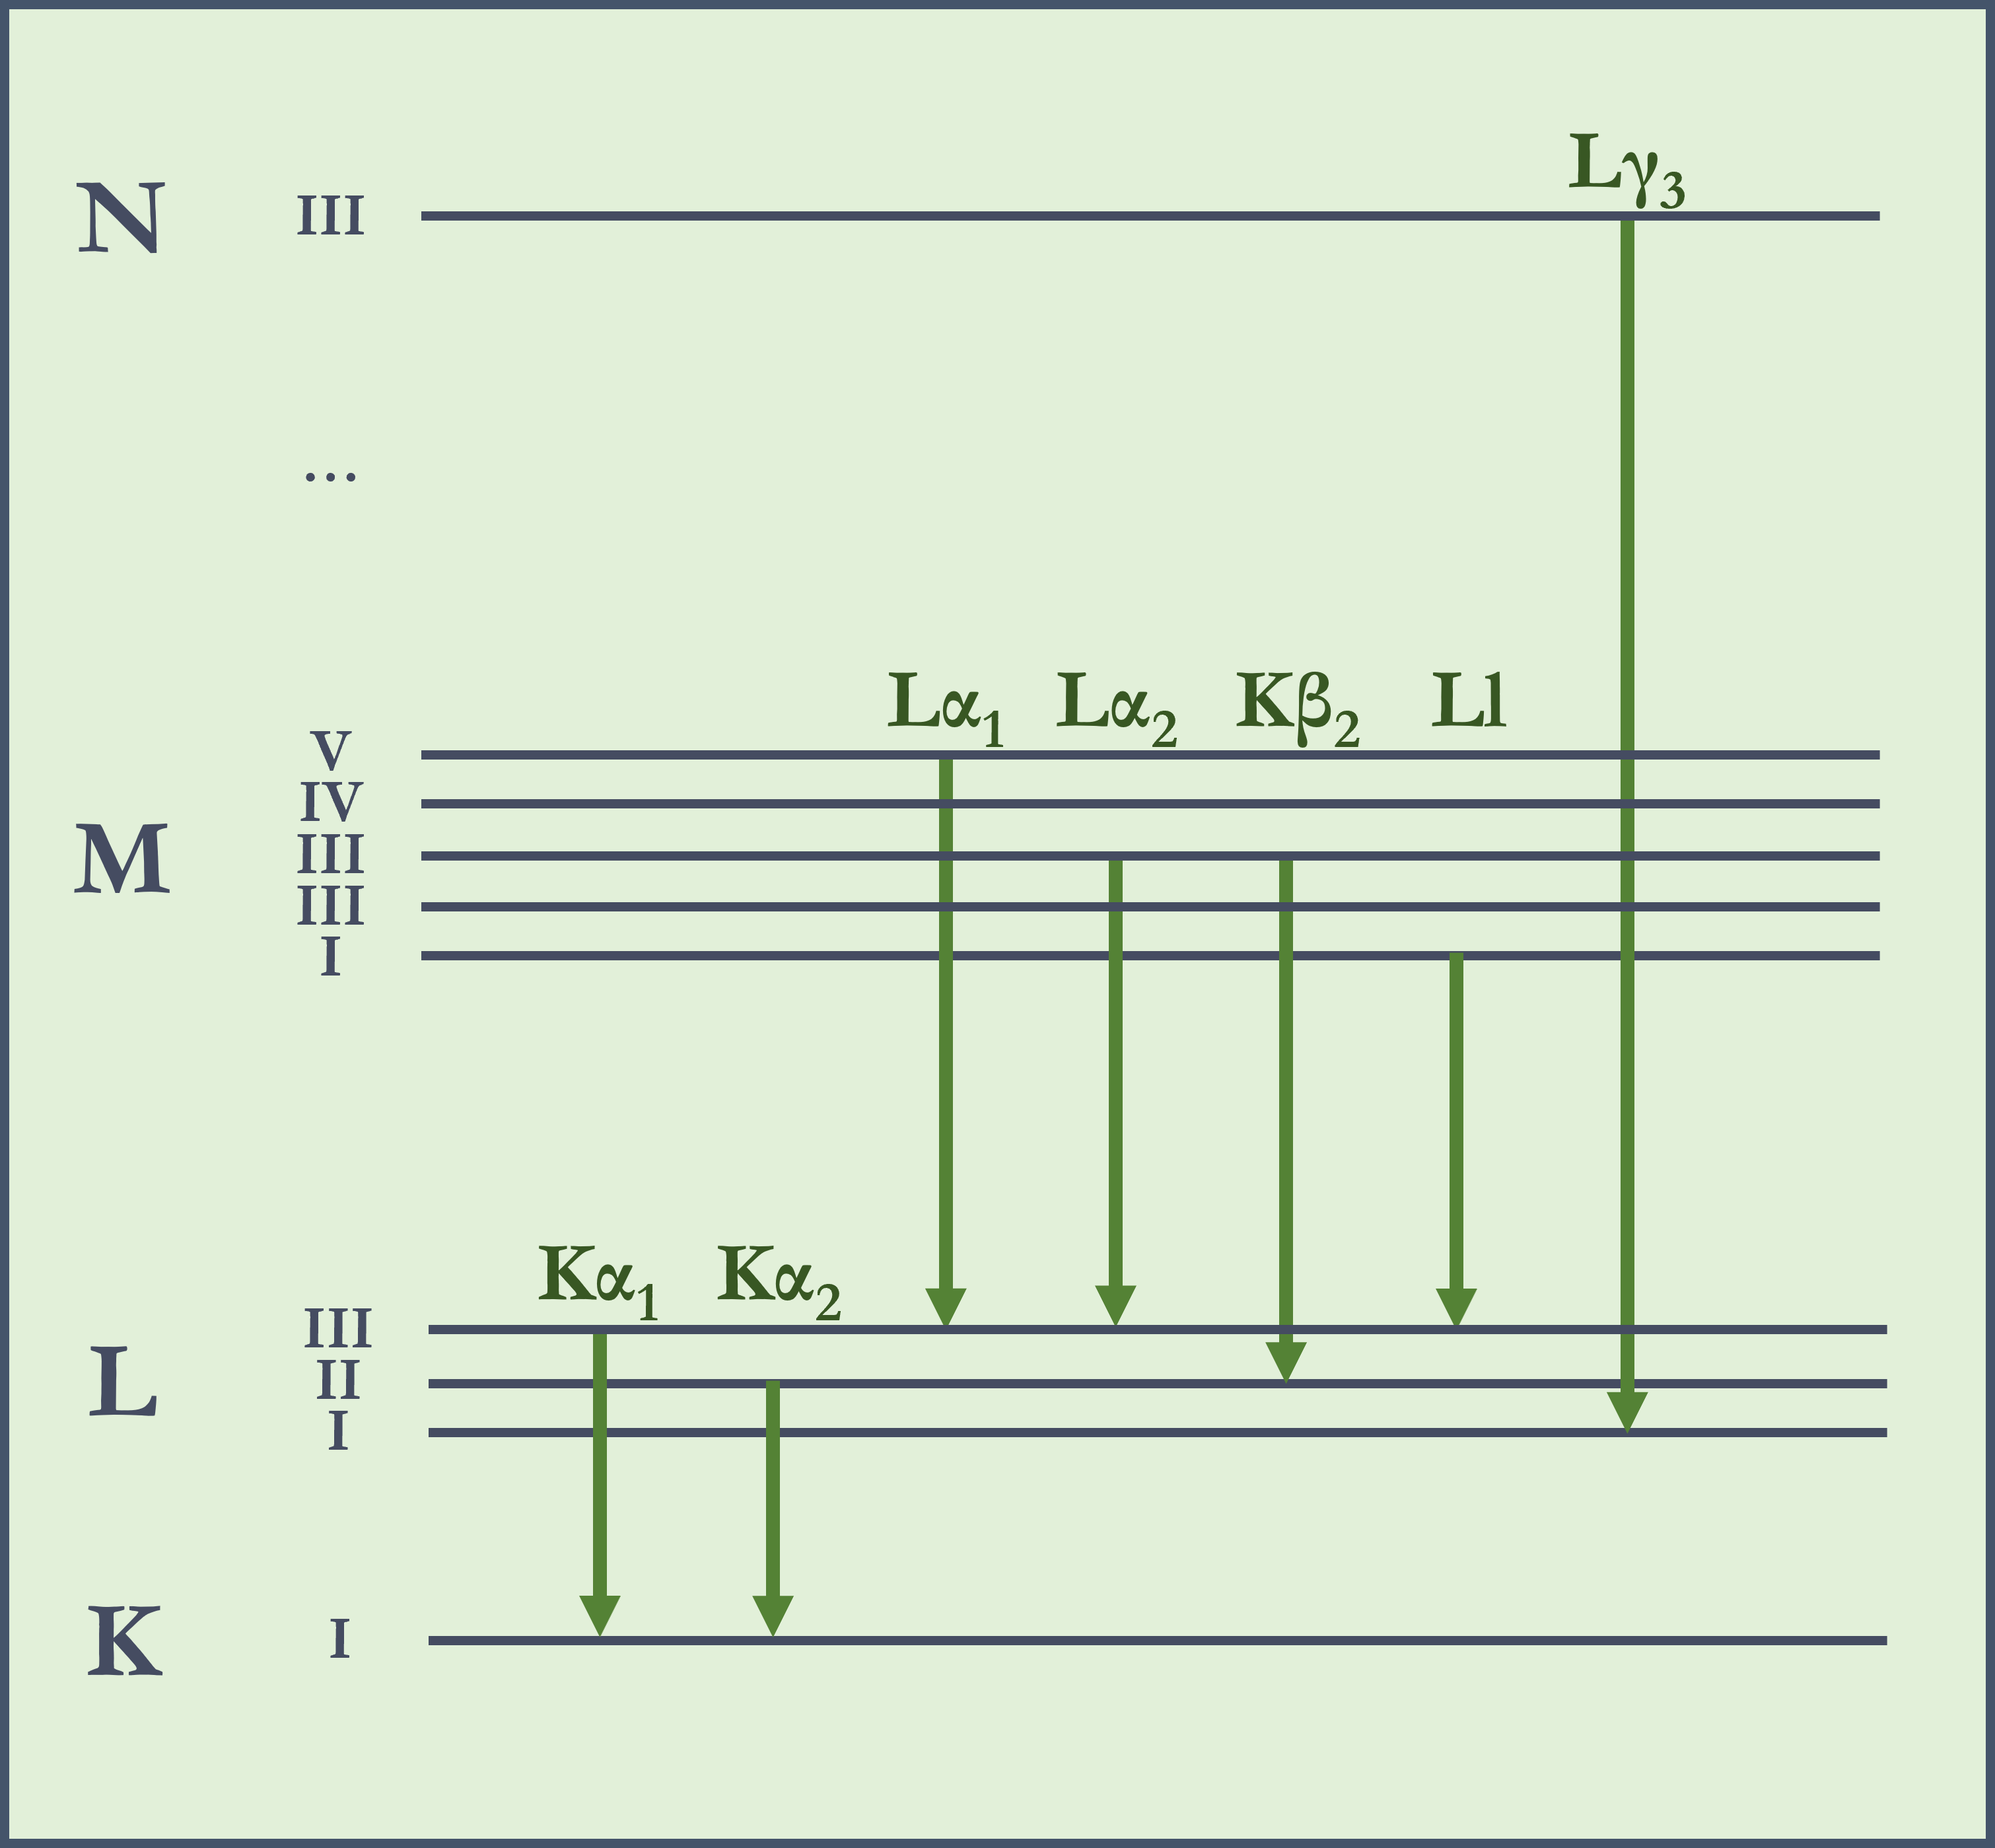
\includegraphics[width=0.7\linewidth]{figures/transition_lines.png}
    \caption{
        Schematic of the electron relaxations relevant for this thesis, with their naming convention.
        The lines are the orbitals in the different shells, and the arrows are the relaxations.
        Quantum number $n$ and $l$ are shown on the right side of the figure.
        The figure also show one forbidden line.
        The distance between the orbitals are increasing with the Z number.
        When the energy of two lines are to close that they are unresolvable, they are referred to as one line, e.g. K$\alpha$1 and K$\alpha$2 are together forming K$\alpha$.
        For Ga, K$\alpha$ = 9.25 keV, K$\beta$ = 10.26 keV and L$\alpha$ = 1.01 keV.
    }
    \label{fig:theory:theoreticalxray:naming:lines}
\end{figure}

% K, L, M
The X-rays are first named by which shell in the Bohr model the vacancy is in, i.e. the principal quantum number $n$ of the vacancy orbital.
Relaxations to the innermost shell $n=1$ is named K-transitions, relaxations to $n=2$ is L-transitions, relaxations to $n=3$ is M-transitions.

% alpha, beta, gamma
The X-rays are further grouped with Greek letters in families. % $\textnormal{e}^-_{3}$ % need to mention families?
Orbitals close in energy are usually in the same group, which means that electrons in the same shell usually are in the same family.
This naming is non-systematic, but tends to follow a pattern where the transitions labeled $\alpha$ are the lower energy transitions corresponding to the $n+1$ orbitals, and the transitions labeled $\beta$ are the higher energy transitions corresponding to the $n+2$ orbitals.
For example, $\textnormal{L} \rightarrow \textnormal{K}$ are $\alpha$-transitions.

% subscript
In addition, the lines in an X-ray group are labeled with subscript numbers which generally start with the highest intensity. % not always!
This is a splitting of the lines due to different energy levels of the orbitals in the same shell.
The different energy levels are due to the spin-orbit coupling, which is the interaction between the electron spin and the orbital angular momentum.
The spin-orbit coupling increase with increased Z, which separates the lines more and more.
The splitting of the $\alpha$ family to $\alpha_1$ and $\alpha_2$ are usually first resolvable in EDS for elements heavier than tin with $ Z = 50$ \cite[Ch. 8.2.2.3]{hollas_modern_2004}. %, where the $\Delta E = 227.3$ eV.

% total naming with example
Putting these three naming conventions together, we name the transition $\textnormal{L}_3 \rightarrow \textnormal{K}_1$ as K$\alpha_1$, and $\textnormal{L}_2 \rightarrow \textnormal{K}_1$ as K$\alpha_2$, with more examples in \cref{fig:theory:theoreticalxray:naming:lines}.
The transition $\textnormal{L}_1 \rightarrow \textnormal{K}_1$ has $\Delta l = 0$ and is thus forbidden by the selection rules, see \cref{eq:theory:theoreticalxray:energyintensity:selectionrules}.
In gallium the K$\alpha_1 = 9251.74$ eV and K$\alpha_2 = 9224.82$ eV \cite{thompson_x-ray_2004} are coupled, but as shown in \cref{fig:results:Ga-K} this energy difference of $\Delta E = 26.92$ eV is too low to be resolved in EDS.














% energy and intensity
\subsection{Energy and intensity}
\label{sec:theory:theoreticalxray:energyintensity}

% short about the energy of the characteristic X-rays
The energy of the characteristic X-ray depends on which orbital the vacancy is in, which orbital the electron is relaxed from, and the amount of protons in the core of atom A. % $\textnormal{e}^-_{3}$ 
Higher Z means higher energy of the characteristic X-ray line, because the energy difference between the relaxation orbital and the ionized orbital is larger.
Atoms with higher Z have more possible transitions, because they have more  electrons and orbitals.

%selection rules
The selection rules, which govern the allowed transitions for the formation of characteristic X-rays, are based on the Pauli exclusion principle and the spin-orbit coupling.
See \cref{fig:theory:theoreticalxray:energyintensity:quantumnumbers} for illustration of the quantum number $n$ and $l$ which are relevant for the selection rules.
Quantum number $j$ is the total angular momentum, which is the sum of the orbital angular momentum $l$ and the spin angular momentum $s$.
The selection rules in \cref{eq:theory:theoreticalxray:energyintensity:selectionrules} is for the electron which relaxes to the vacancy in the core orbital of atom A \cite[Sec. 8.2.2.2]{hollas_modern_2004}.

\begin{equation}
    \label{eq:theory:theoreticalxray:energyintensity:selectionrules}
    \Delta n \ge 1;\qquad \Delta l  = \pm 1;\qquad \Delta j = 0, \pm 1
\end{equation}

% figure from wikipedia showing n, l, j
% file: wikipedia-quantum-numbers-n-l-j.png
\begin{figure}[p]
    \centering
    % \captionsetup{0.8\linewidth}
    % remove \colorbox to get the figure transparent again
    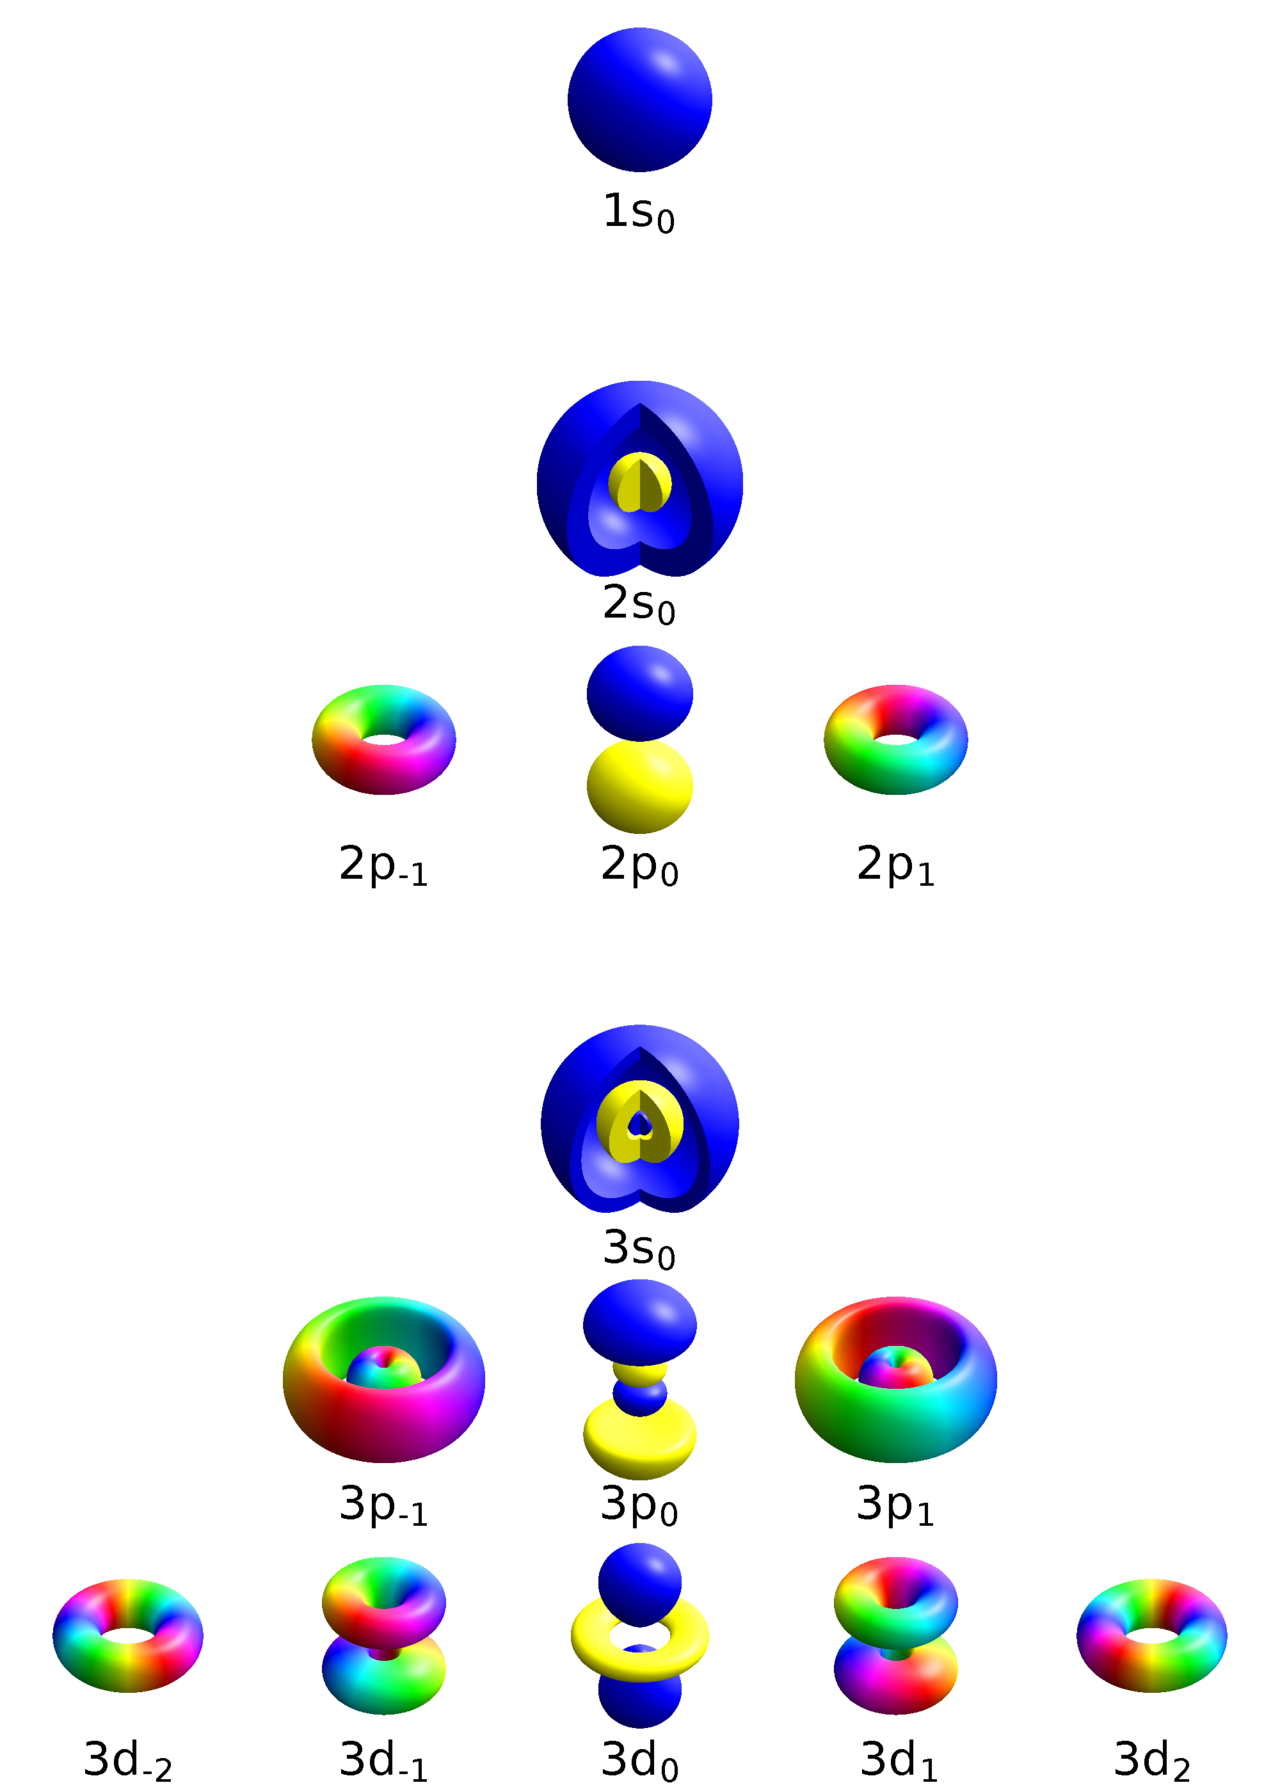
\includegraphics[width=0.8\linewidth]{figures/wikipedia-quantum-numbers-n-l-j.png}
    \caption{
        The quantum numbers $n$, $l$, and $m$ in a hydrogen-like atom.
        The principal quantum number is shown as the block with values $n= 1, 2, 3$.
        The Azimuthal quantum number is the rows as $l = s, p, d$, where their numbers are 0, 1 and 2.
        The magnetic quantum number is the columns as $m = -2, -1, 0, 1, 2 $.
        The spin quantum number, $s$, is not geometrically independent.
        The total angular momentum quantum number $j = l + s$, and since $s$ is geometrically independent it is not possible to visualize $j$ here.
        The figure is an altered version of a figure from the article "Quantum number" on Wikipedia, made by Geek3 - Own work, Created with hydrogen 1.1, CC BY-SA 4.0, \url{https://commons.wikimedia.org/w/index.php?curid=67681892}.
    }
    \label{fig:theory:theoreticalxray:energyintensity:quantumnumbers}
\end{figure}


% intensity in theory
Even though heavy atoms like gold have more than 30 possible transitions, only a few are detectable in EDS.
Lines which are undetectable have low abundance, are too close to other lines, or are forbidden by the selection rules \cite[Ch. 4.2.3]{goldstein_scanning_2018}.
Lines which are detectable have an intensity dependent on the amount of the element in the sample, because a higher amount gives more counts in the detector.
The counts in EDS the number of X-ray photons detected in a specific energy range.
The energy range is typically around 10 eV.
In theory, the ratio of the atomic concentration between two elements are proportional to the ratio of the corresponding lines from the elements.
However, there are many factors which affect the intensity of the lines, which are covered in \cref{sec:theory:empirical}.
A theoretical spectrum with just lines are shown in \cref{fig:theory:expected_lines}.
The lines are not spread, and have different energy and intensity.
Am other illustration of a theoretical spectrum, but with a background radiation, is shown in \cref{fig:theory:expected_spectrum_Skomedal}.
The background radiation is generated exponentially, but at lower energies the background radiation is absorbed and thus get the illustrated shape.
A real spectrum is shown in \cref{fig:theory:actual_peaks}.
In this figure the lines are spread, and there is a background present which is low.
The shape of a real background is shown in \cref{fig:theory:expected_background}.
Both \cref{fig:theory:actual_peaks,fig:theory:expected_background} have counts on the y-axis.


% figure figures/expected_lines.png
\begin{figure}[p]
    \centering
    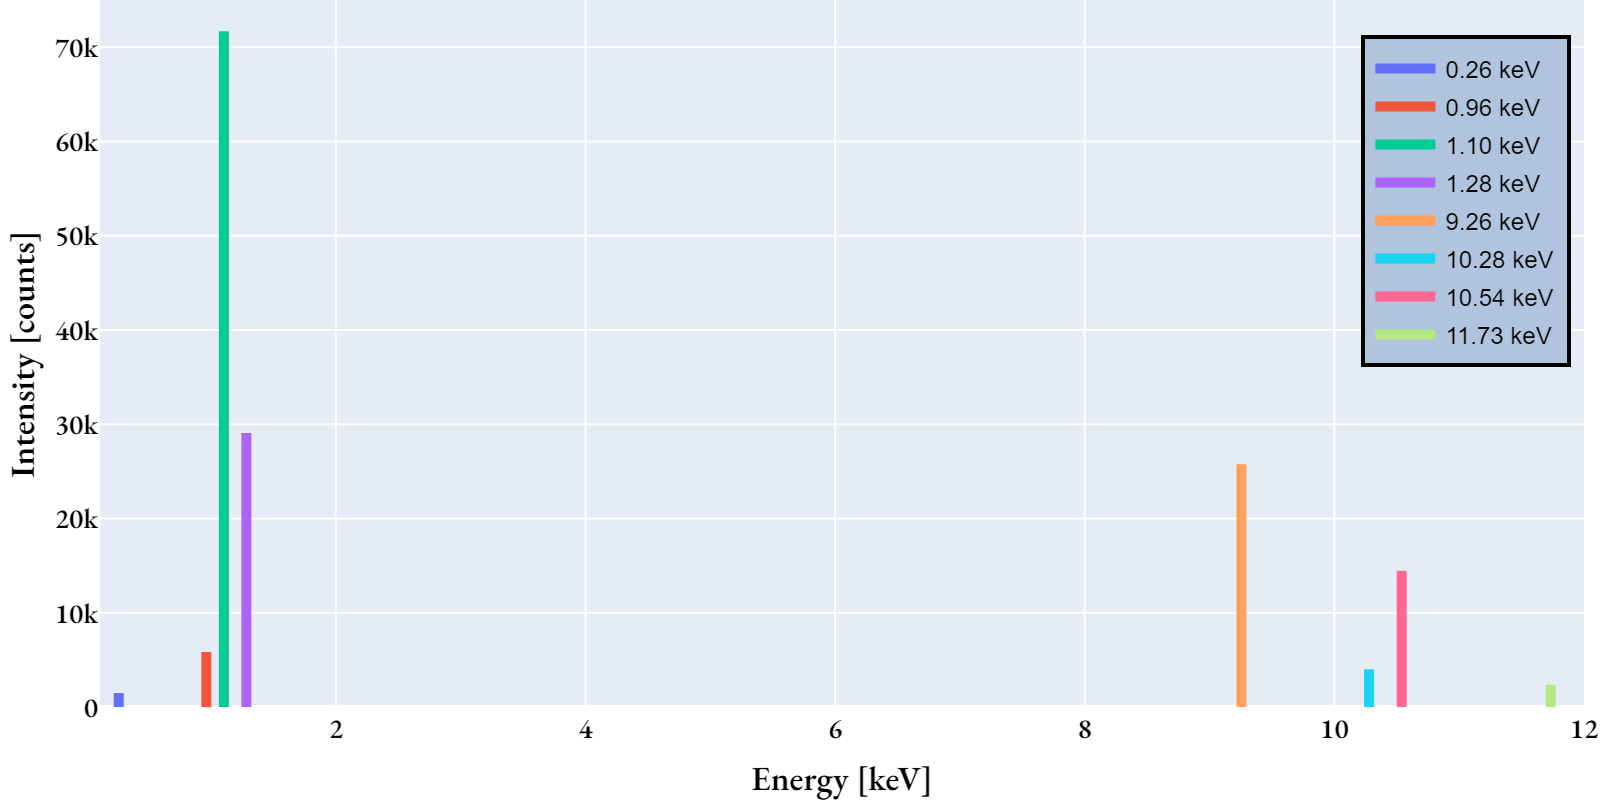
\includegraphics[width=0.9\textwidth]{figures/expected_lines.png}
    \caption{
        Theoretical lines in a spectrum.
        The lines have different energy and intensity.
    }
    \label{fig:theory:expected_lines}
\end{figure}

% figure/expected_spectrum_Skomedal.png
\begin{figure}[p]
    \centering
    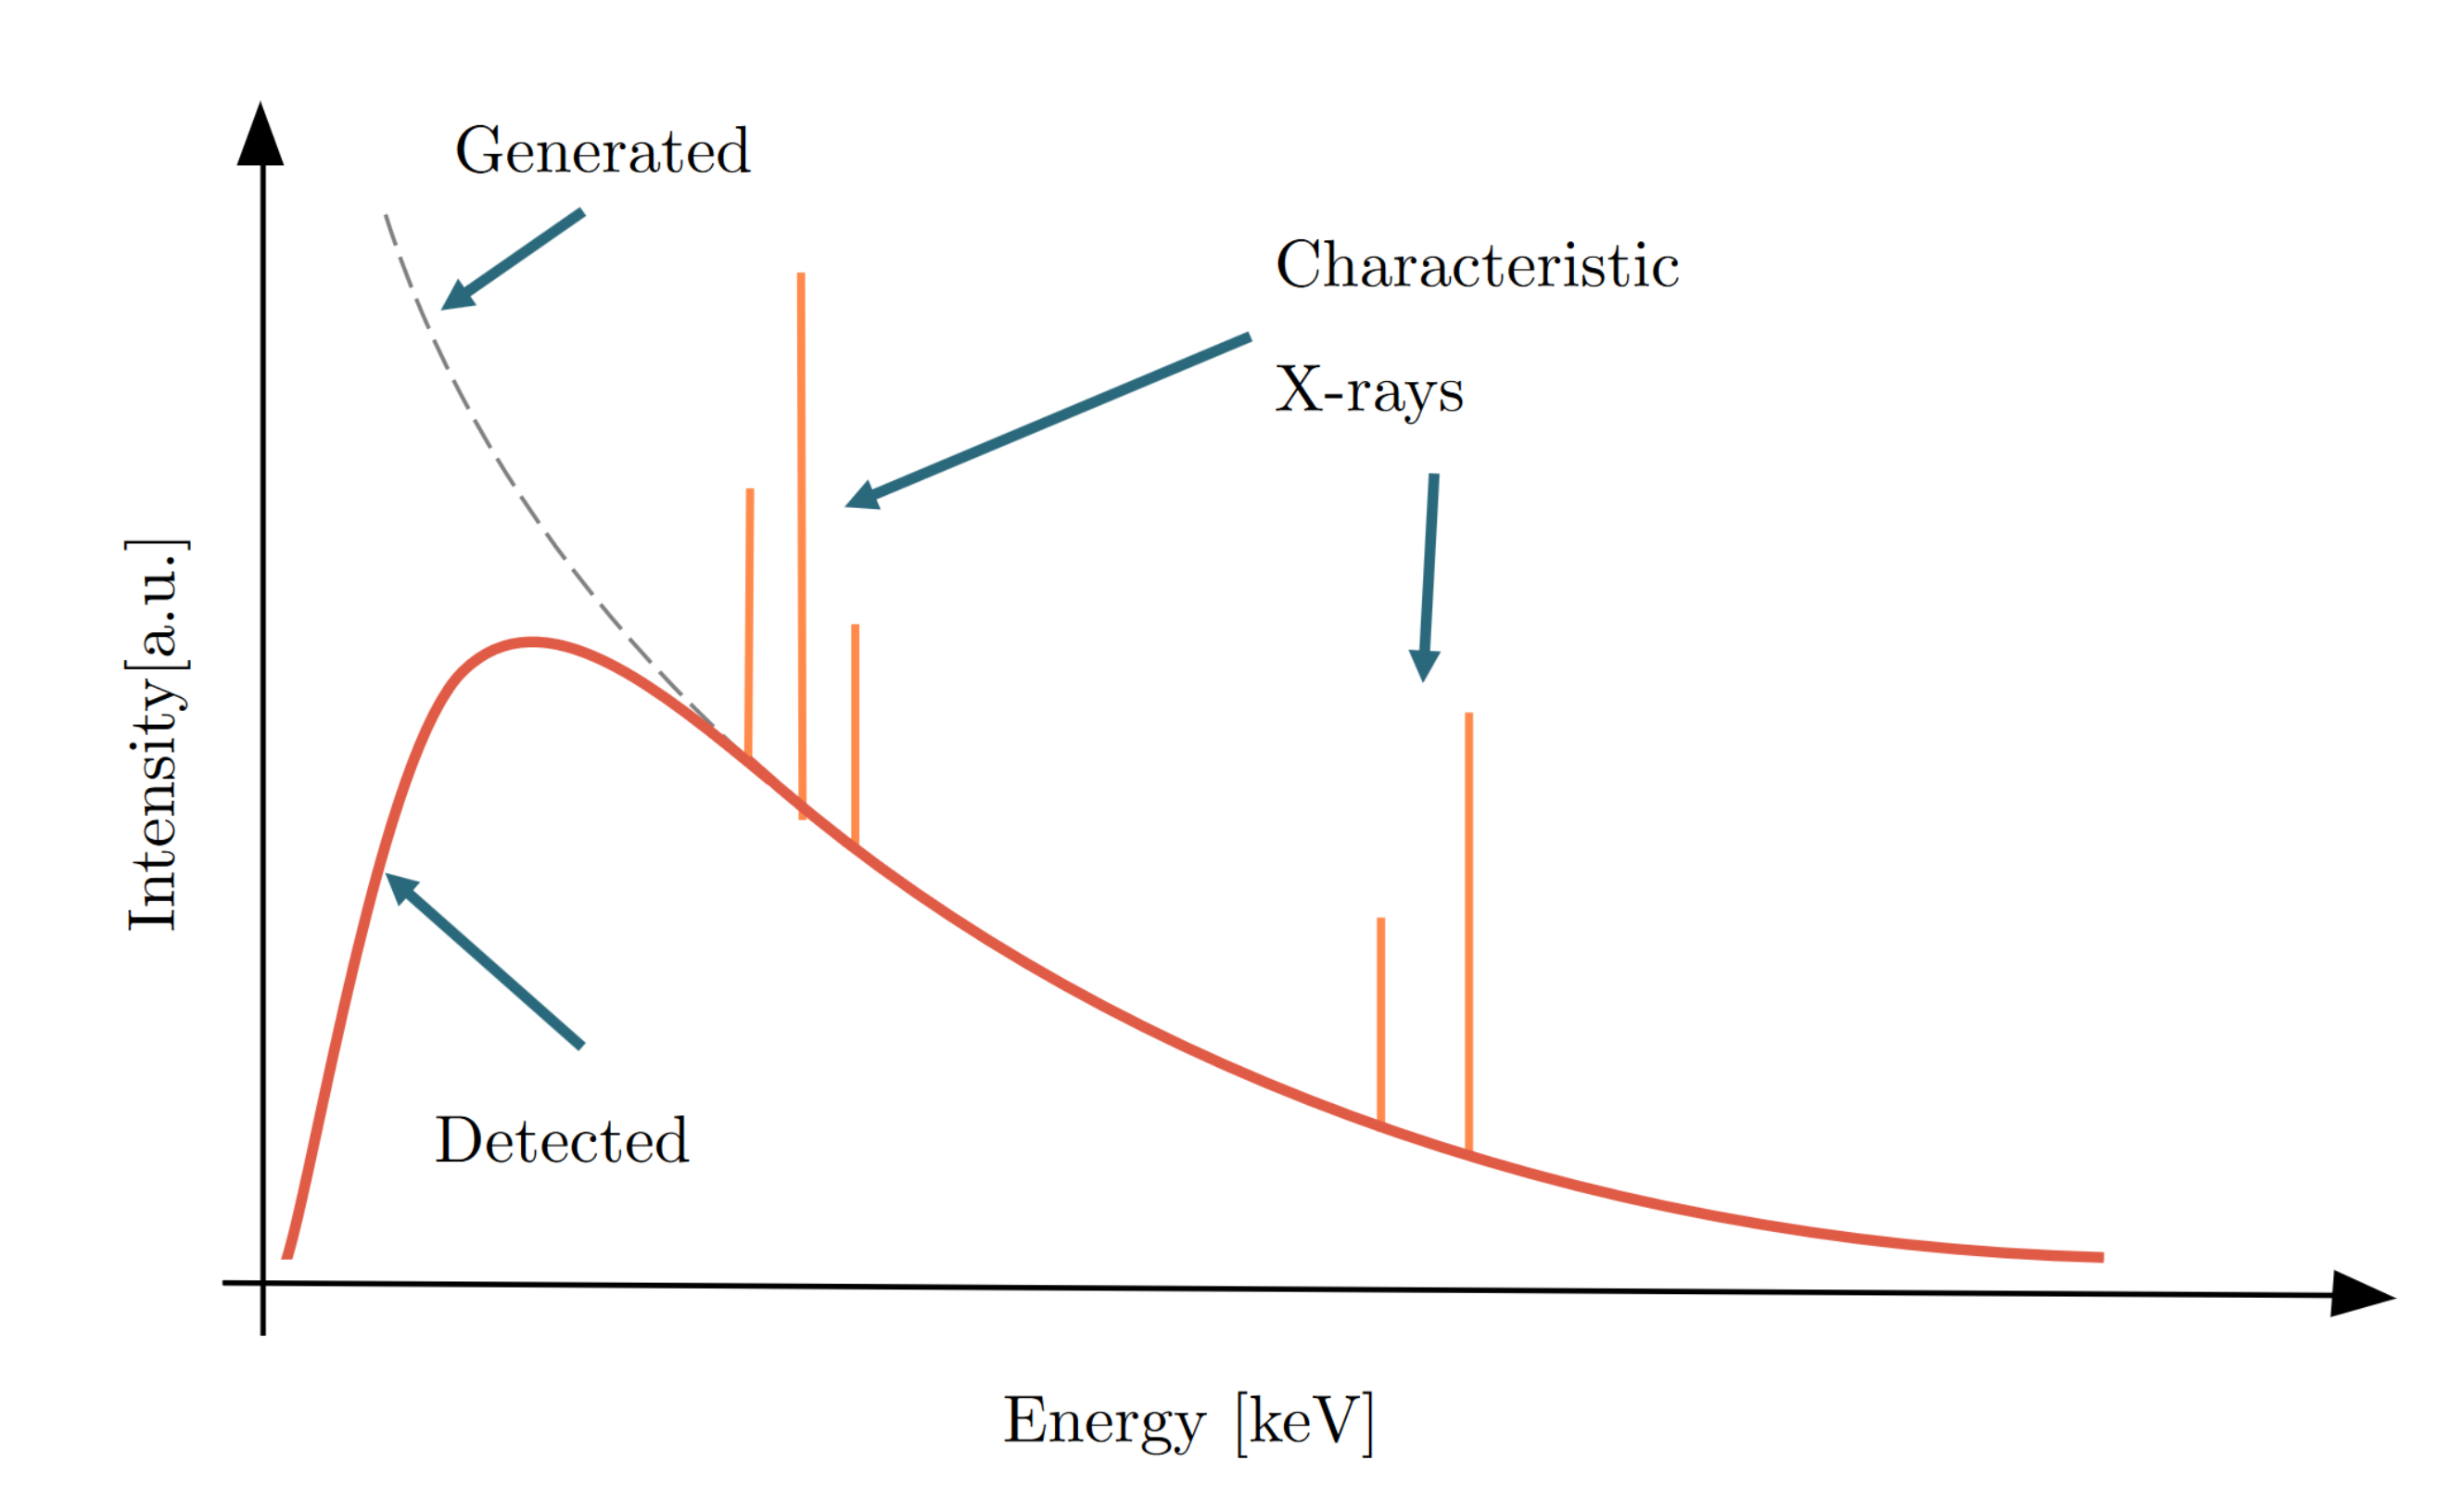
\includegraphics[width=0.9\textwidth]{figures/expected_spectrum_Skomedal.png}
    \caption{
        An illustration of a theoretical spectrum with characteristic X-rays and background radiation.
        The background radiation is being generated exponentially, but lower energies the X-rays are absorbed, and thus the detected background get the illustrated shape.
        The figure is borrowed from Skomedal \cite[Fig. 2.8]{skomedal_improving_2022}.
    }
    \label{fig:theory:expected_spectrum_Skomedal}
\end{figure}


% figure/acutal_peaks.png
\begin{figure}[p]
    \centering
    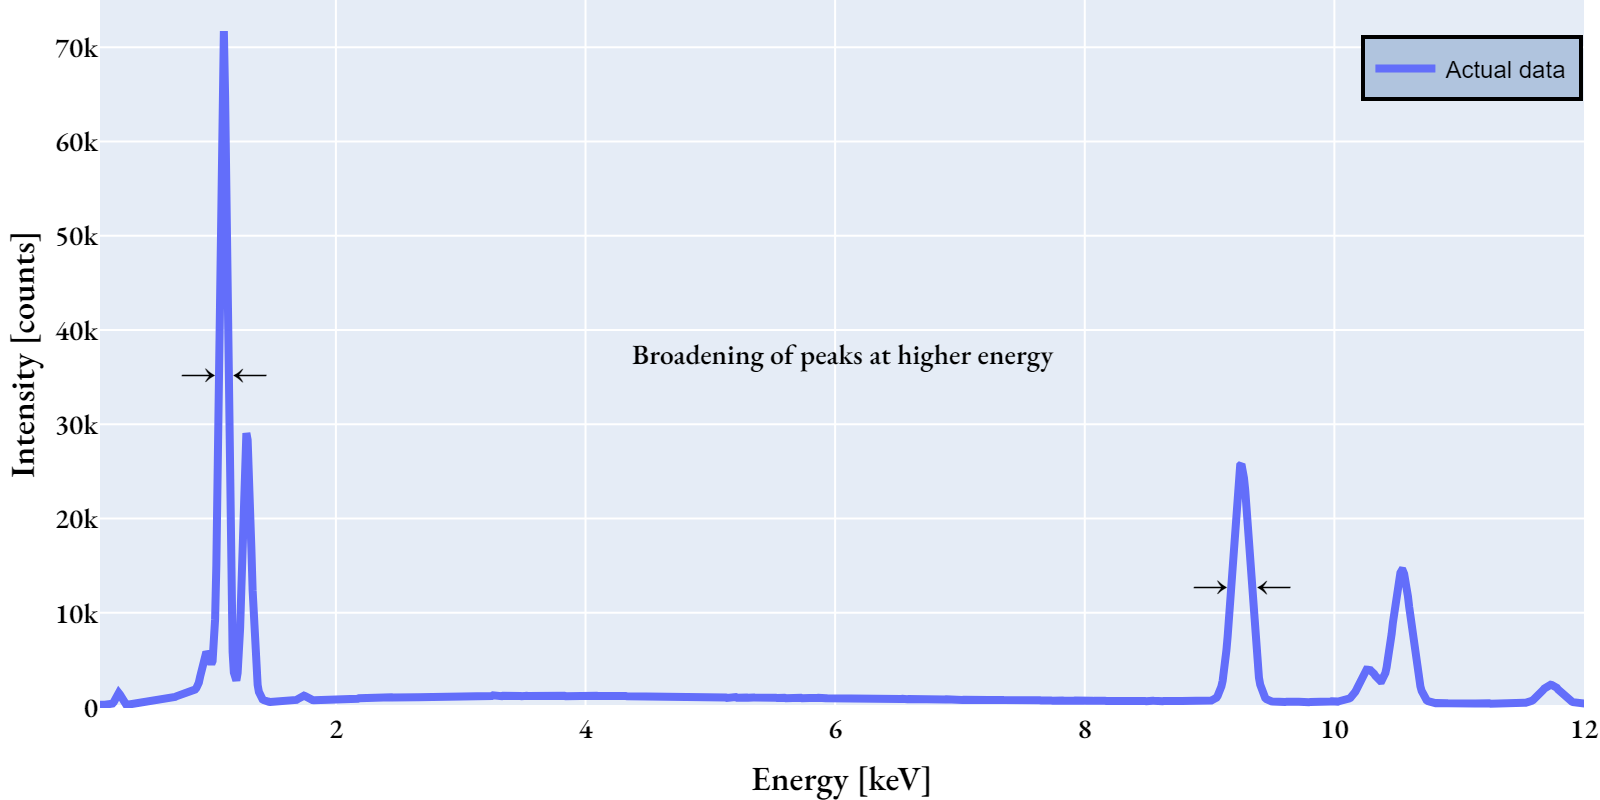
\includegraphics[width=0.9\textwidth]{figures/actual_peaks.png}
    \caption{
        Actual lines, or peaks, in a spectrum.
        The lines have different energy and intensity, and they have a spread.
        The peaks have Gaussian shapes, as the formation of characteristic X-rays is a probability process.
        This is a real spectrum with a background, but it is low and do not show.
        A typical background is plotted in \cref{fig:theory:expected_background}.
    }
    \label{fig:theory:actual_peaks}
\end{figure}


% figure/expected_bacground.png
\begin{figure}[p]
    \centering
    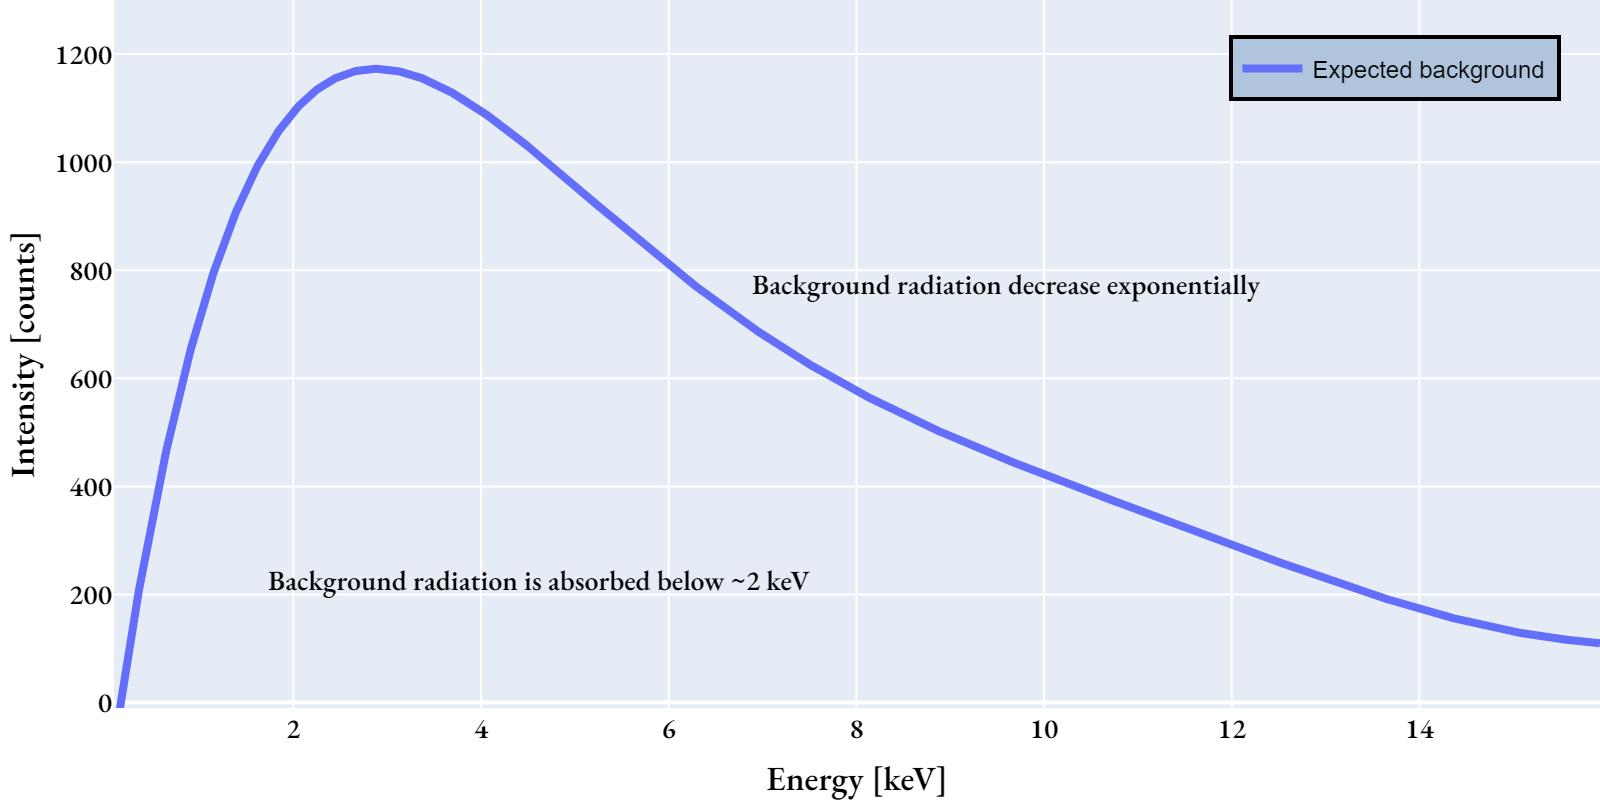
\includegraphics[width=0.9\textwidth]{figures/expected_background.png}
    \caption{
        Expected background in a spectrum.
        This is a fit of a real background spectrum, but the exact numbers are not important.
        The background radiation is being generated exponentially, but at lower energies it is being absorbed.
        The figure is meant to illustrate the shape of the background.
    }
    \label{fig:theory:expected_background}
\end{figure}


% \begin{figure}
%     \centering
%     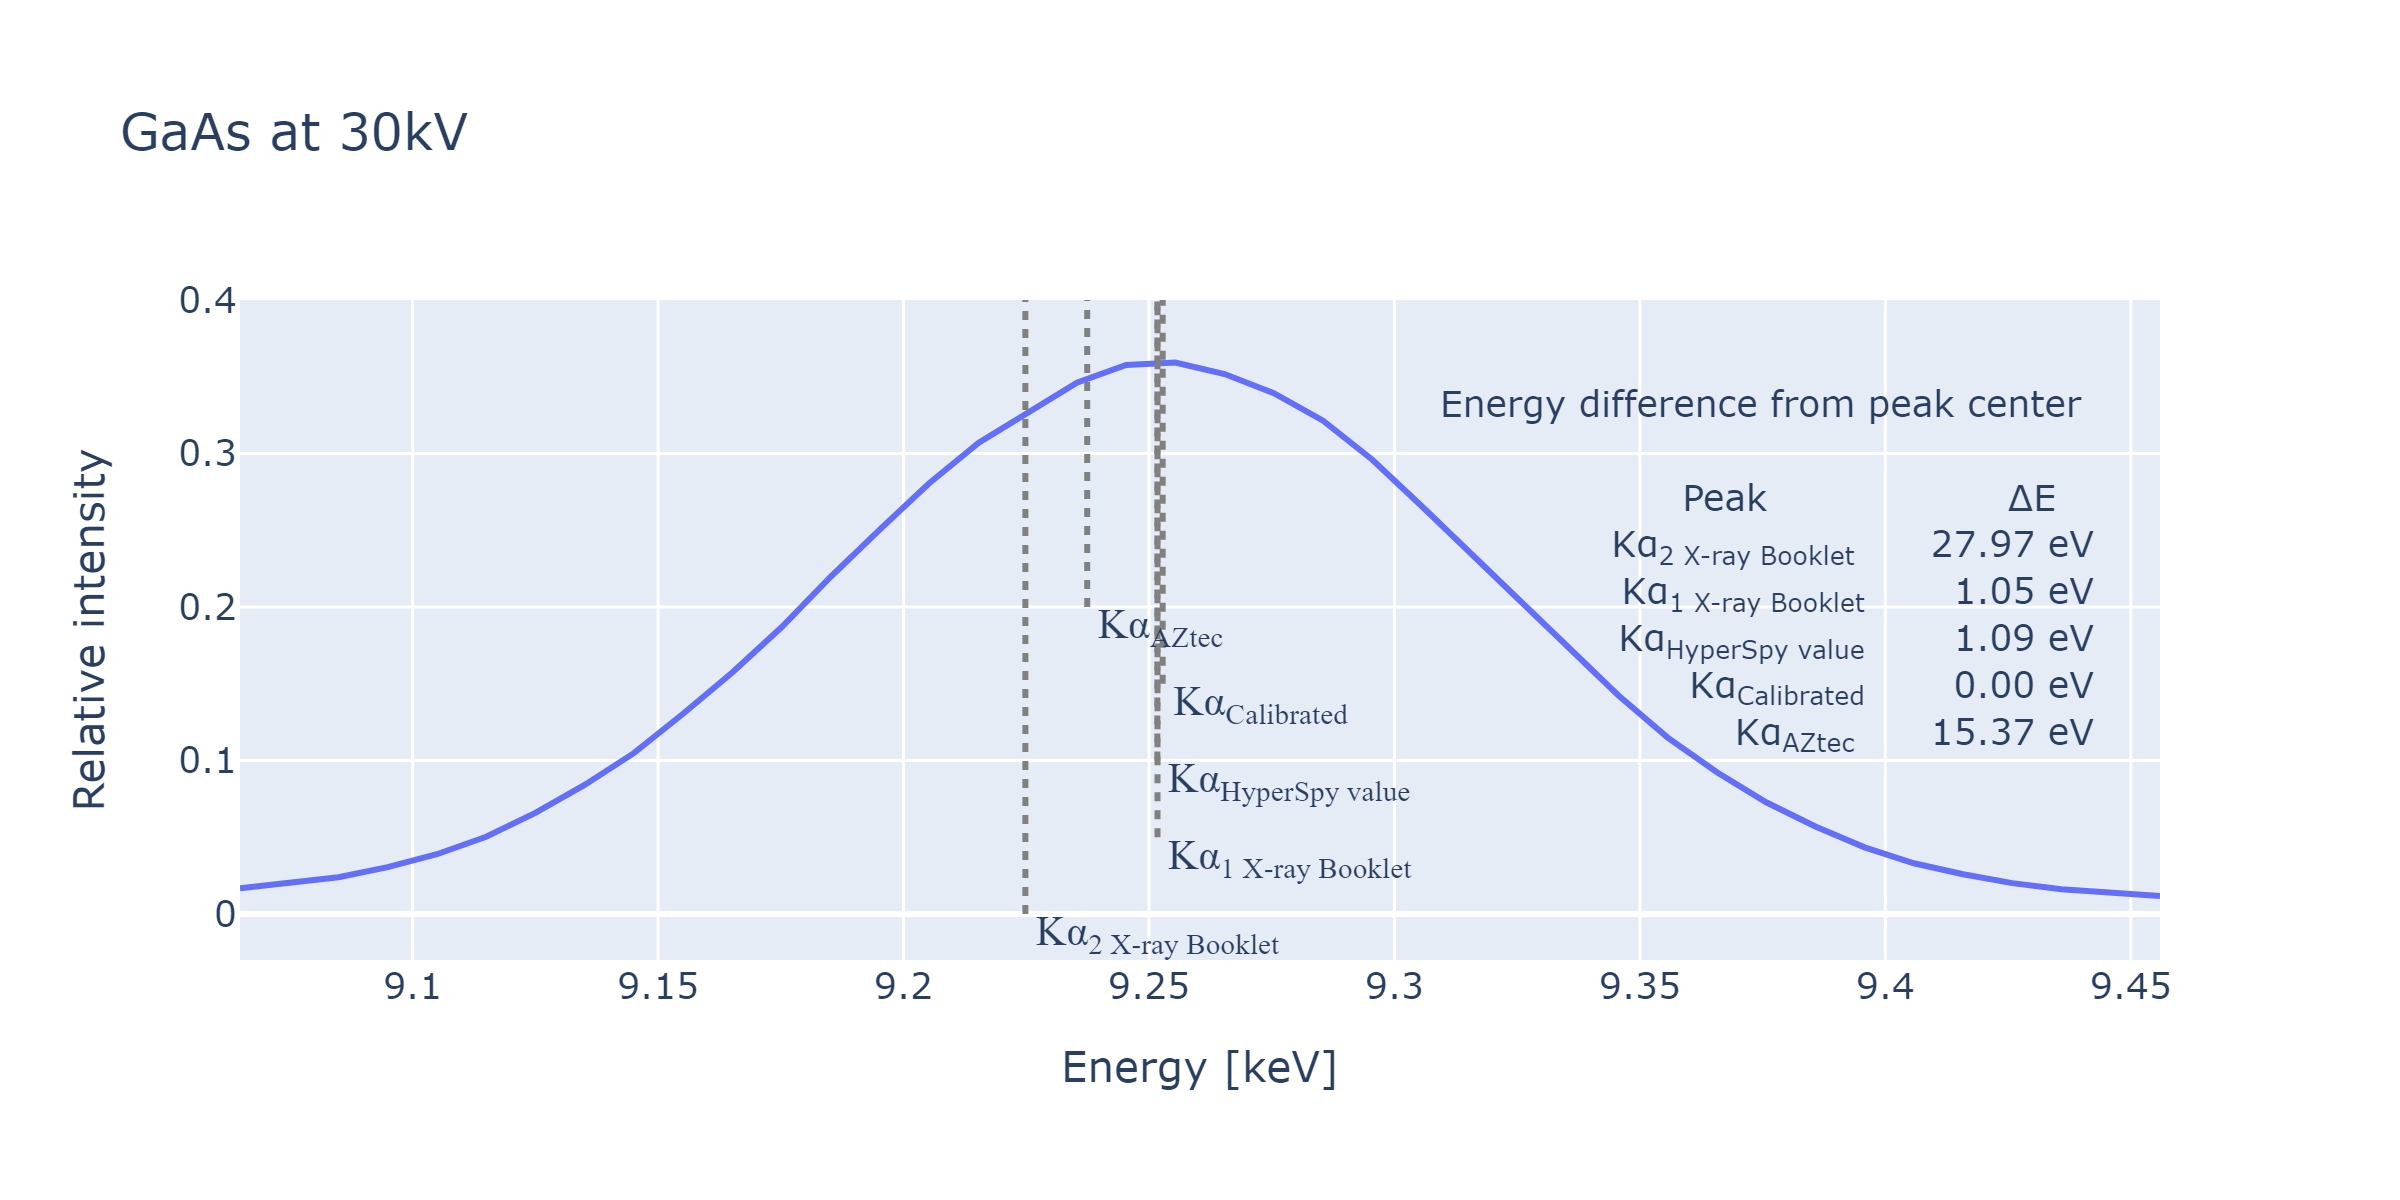
\includegraphics[width=0.9\textwidth]{figures/GaAs30kV-Ga-K-lines.png}
%     \caption{
%         The theoretical lines K$\alpha_1 = 9.25174$ and K$\alpha_2 = 9.22482$ from the X-ray Data Booklet with K$\alpha = 9.251$ from HyperSpy and the fitted peak K$\alpha$.
%         The spectrum is calibrated to Ga $L\alpha$ and As K$\alpha$, where the energy of the peaks is taken from HyperSpy.
%         HyperSpy gives Ga K$\alpha$ almost directly on top of the theoretical K$\alpha_1$.
%         This figure show that the lines which are separated with small energy differences are so close that they make one single peak in the EDS spectrum.
%         Data from the SEM Apreo at NTNU NanoLab, 30kV.
%         \ton{This is more results than theory I would say. But I do remember you saying something about having this in the theory section.}
%     }
%     \label{fig:theory:GaAs30keV-K-lines}
% \end{figure}



% theoretical values of the lines
Theoretical values of characteristic X-ray lines are available in the X-ray Data Booklet \cite{thompson_x-ray_2004} and in HyperSpy \cite{hyperspy_1.7.1}.
These include the energy and the weight of the lines.
All the lines for Ga and Mo are listed in \cref{tab:theory:Ga-lines} and \cref{tab:theory:Mo-lines}.
There are minor differences in the energies and weights from the XRB and HS.
One bigger difference between the two tables is that HyperSpy have a line for Mo L$\gamma$3, which is not in the X-ray Data Booklet.
Another difference is that the X-ray Data Booklet splits the K$\alpha$ line into two lines, while HyperSpy have one line for the K$\alpha$ line.
In addition, the XRB list Mo L$\alpha$ as two lines and Mo K$\beta$ as three lines.
These additional lines are very close in energy and only one of the lines have a higher weight, so these line separations are excluded from the tables.
% include the table in table/Ga-lines.tex
% table listing the Ga lines, both from Hyperspy and from the X-ray booklet

\begin{table}[tbp]
    \centering
    \caption{
        Ga lines from HyperSpy cite ?? and X-ray booklet \cite{thompson_x-ray_2004}.
        ** HyperSpy operates with a single line for each K and L shell, but the X-ray booklet lists two lines for each shell.
        * HyperSpy lists Ln, Ll and L$\beta_3$ as separate lines, but I am not sure what they correspond to in the X-ray booklet.
        TODO: Figure out this.
    }
    \label{tab:theory:Ga-lines}
    \begin{tabular}{llll}
                       & X-ray booklet & HyperSpy     & HyperSpy \\
                       & Energy [keV]  & Energy [keV] & Weight   \\
        \hline
        K$ \alpha_1$   & 9.25174       & 9.2517       & 1.0      \\
        K$ \alpha_2$** & 9.22482       &              &          \\
        K$ \beta_1$    & 10.2642       & 10.2642      & 0.1287   \\
        L$ \alpha_1$   & 1.09792       & 1.098        & 1.0      \\
        L$ \alpha_2$** & 1.09792       &              &          \\
        L$ \beta_1$    & 1.1248        & 1.1249       & 0.16704  \\
        L$n$*          &               & 0.9843       & 0.02509  \\
        L$l$*          &               & 0.0544       & 0.9573   \\
        L$b_3$*        &               & 0.0461       & 1.1948
    \end{tabular}

\end{table}

% table listing the Mo lines, both from Hyperspy and from the X-ray Data Booklet

\begin{table}[tbp]
    \centering
    \caption{
        Mo lines from the HyperSpy library \cite{hyperspy_1.7.1} and X-ray Data Booklet (XRB) \cite[Table 1.2 and 1.3]{thompson_x-ray_2004}.
        HyperSpy lists a single line for K$\alpha$, while the XRB lists two lines.
        The weights are relative to the strongest line in each shell for each element.
        HyperSpy include a line at 2.83 keV for Mo L$\gamma$3, which is not listed in the XRB.
        HyperSpy also include a line at 2.47 keV for Mo L$\beta$3, which is not listed in the XRB.
    }
    \label{tab:theory:Mo-lines}
    \begin{tabular}{cccccc}
        Line       & XRB          & XRB    & HyperSpy     & HyperSpy \\
                   & Energy [keV] & Weight & Energy [keV] & Weight   \\
        \hline
        L$\beta$1  & 2.3948       & 0.53   & 2.3948       & 0.33     \\
        K$\beta$   & 19.608       & 0.15   & 19.6072      & 0.15     \\
        K$\alpha$  & 17.4793      & 1.0    & 17.4793      & 1.0      \\
        K$\alpha$2 & 17.3743      & 0.52   &              &          \\
        L$\beta$2  & 2.5183       & 0.05   & 2.5184       & 0.05     \\
        L$\alpha$  & 2.2932       & 1.0    & 2.2932       & 1.0      \\
        % Ln         &              &        & 2.1205       & 0.01     \\
        Ll         & 2.0157       & 0.05   & 2.0156       & 0.04     \\
        L$\beta$3  &              &        & 2.4732       & 0.06     \\
        L$\gamma$3 &              &        & 2.8307       & 0.01     \\
        L$\gamma$1 & 2.6235       & 0.03   & 2.6233       & 0.01
    \end{tabular}
\end{table}

\clearpage











\section{Empirical view on characteristic X-rays}
\label{sec:theory:empirical}
On top of the theoretical physics there are many experimental processes affecting both the creation and the detection of characteristic X-rays.
The scientific community uses an empirically influenced approach in EDS analysis.
This approach includes empirical equations to deal with atomic number effects, absorption in the sample, secondary scattering or fluorescence, the imperfect beam, scattering in the chamber, several cross sections and the imperfect detector.
There are many processes that can and do happen which complicates the physics.
The easy view is just to analyze the signal and do not worry too much about the physics behind it.
This is the empirical way.

% \ton{What do I do with the thin film assumptions? How do I mention it?}
% this is related to quantification, that absorption and eventual fluorescence can be ignored as they are not significant. That makes analysis easier. Not relevant for formation, there want that probe is absorbed, so thick.
% Could say that there are many processes that can happen (several cross sections). The easy view is just look at what comes out at end.

%
%
%   - from lines to peaks
%     - broadening of line to peaks
%     - peak shape, gaussian
\subsection{From lines to peaks}
\label{sec:theory:empirical:peaks}
A striking difference between the theoretical and the empirical view is that the lines are not lines, but peaks with a varying width.
This is illustrated in \cref{fig:theory:expected_lines} and \cref{fig:theory:actual_peaks}.
The peaks in the EDS spectrums have a Gaussian shape, which is a result of the signal being a statistical distribution of the electronically detected X-rays.
\cref{fig:theory:actual_peaks} shows that lower energy lines are narrower than higher energy lines.
The electronics in the detector are broadening the lines, and each detector has its own broadening function \cite{broadening_broduscha}.

As the peaks are broadened, every peak in the spectrum can be fitted with a Gaussian function.
A Gaussian peak is a curve defined by the following equation:

\begin{equation}
    \label{eq:theory:empirical:gaussian}
    g(x) = \frac{1}{\sigma \sqrt{2\pi}} exp({-\frac{(x-\mu)^2}{2\sigma^2}})
\end{equation}

In the equation $\mu$ is the center of the peak, $\sigma$ is the standard deviation, and $x$ is the energy.
When doing peak fitting, the first term is treated as the amplitude and is a parameter which is fitted, i.e. $1/\sigma\sqrt{2\pi}$ is swapped with a parameter $A$.
The three fitted parameters are $\mu$ (center of the peak), $\sigma$ (standard deviation) and $A$ (amplitude).
$x$ is the energy, i.e. the x-axis in the EDS spectrum.

The width of the peak is a measure of the broadening of the line, and is usually given as the FWHM in EDS analysis. The FWHM is connected to the standard deviation of the Gaussian distribution, which is given by \cref{eq:theory:empirical:gaussian}.
The FWHM can be calculated from the standard deviation, $\sigma$, with:

% Eq FWHM
\begin{equation}
    \label{eq:theory:empirical:peaks:FWHM}
    \textnormal{FWHM} = {\sigma}{2\sqrt{2\ln(2)}}
\end{equation}


%
% 
%   - intensities
%     - weight of a line intro
%     - fluorescent yield approx
%     - empirical weights in HyperSpy,
%     - k-factor
%     - k-ratio
\subsection{Intensity}
\label{sec:theory:empirical:intensity}

% intensity in reality
% put this in the empirical section, just say that it is lower for low energy because of many reasons (absorption, efficiency). Same reason than background is lower for low energy. 

% remove?
% After the first relaxation there is also an avalanche of following relaxation events to the new hole in the relaxed orbital.
% All but the first relaxation are too low in energy to be detected as characteristic X-rays in EDS.

% weight of a line
The intensity, or weight, of a line is dependent on multiple empirical and physical factors.
This subsection will briefly cover fluorescent yield, critical ionization energy, and empirical weights in HyperSpy.
In practice, the weight of the lines are included as a part of the k-factors or k-ratios, which are presented in \cref{sec:theory:empirical:kfactors}.
Only the strongest lines are listed in the X-ray Data Booklet, where the theoretical values of the characteristic X-ray lines are listed.
The list include: K$\alpha_1$, K$\alpha_2$, K$\beta_2$, L$\alpha_1$, L$\alpha_2$, L$\beta_1$, L$\beta_2$, L$\gamma_1$, M$\alpha_1$ \cite{thompson_x-ray_2004}.
HyperSpy have a library of the X-ray lines of the elements too.
The X-ray lines which were identified in this project are illustrated in \cref{fig:theory:theoreticalxray:naming:lines}.












% fluorescent yield
The fluorescent yield $\omega$ is non-linearly dependent on $Z$.
Figure (4.3) in Goldstein \cite{goldstein_scanning_2018} is copied in \cref{fig:theory:fluorescence_yield}, which shows that the fluorescent yield for the first 90 elements is mostly increasing with $Z$.
For K- and L-shell fluorescent yield, $\omega$ is strictly increasing.
For M-shell fluorescent yield, $\omega$ is strictly increasing till around $Z=80$, and then it starts to decrease.
The figure also show that for the same element $\omega_{\textnormal{K}}  > \omega_{\textnormal{L}} > \omega_{\textnormal{M}}$.
When dealing with thin samples, the fluorescent yield can be approximated by an empirical formula based on tin.
The formula is given in \cref{eq:empirical:fluorescentyieldapprox}, where $a=10^6$ for K-shell.
The two key takeaways from this formula is that $\omega$ is dependent on $Z$, but kinda similar for close elements like Ga $Z = 31$ and As $Z = 33$.

% figure/fluorescence_yield_Goldstein_Fig4.3.d.png
\begin{figure}[h]
    \centering
    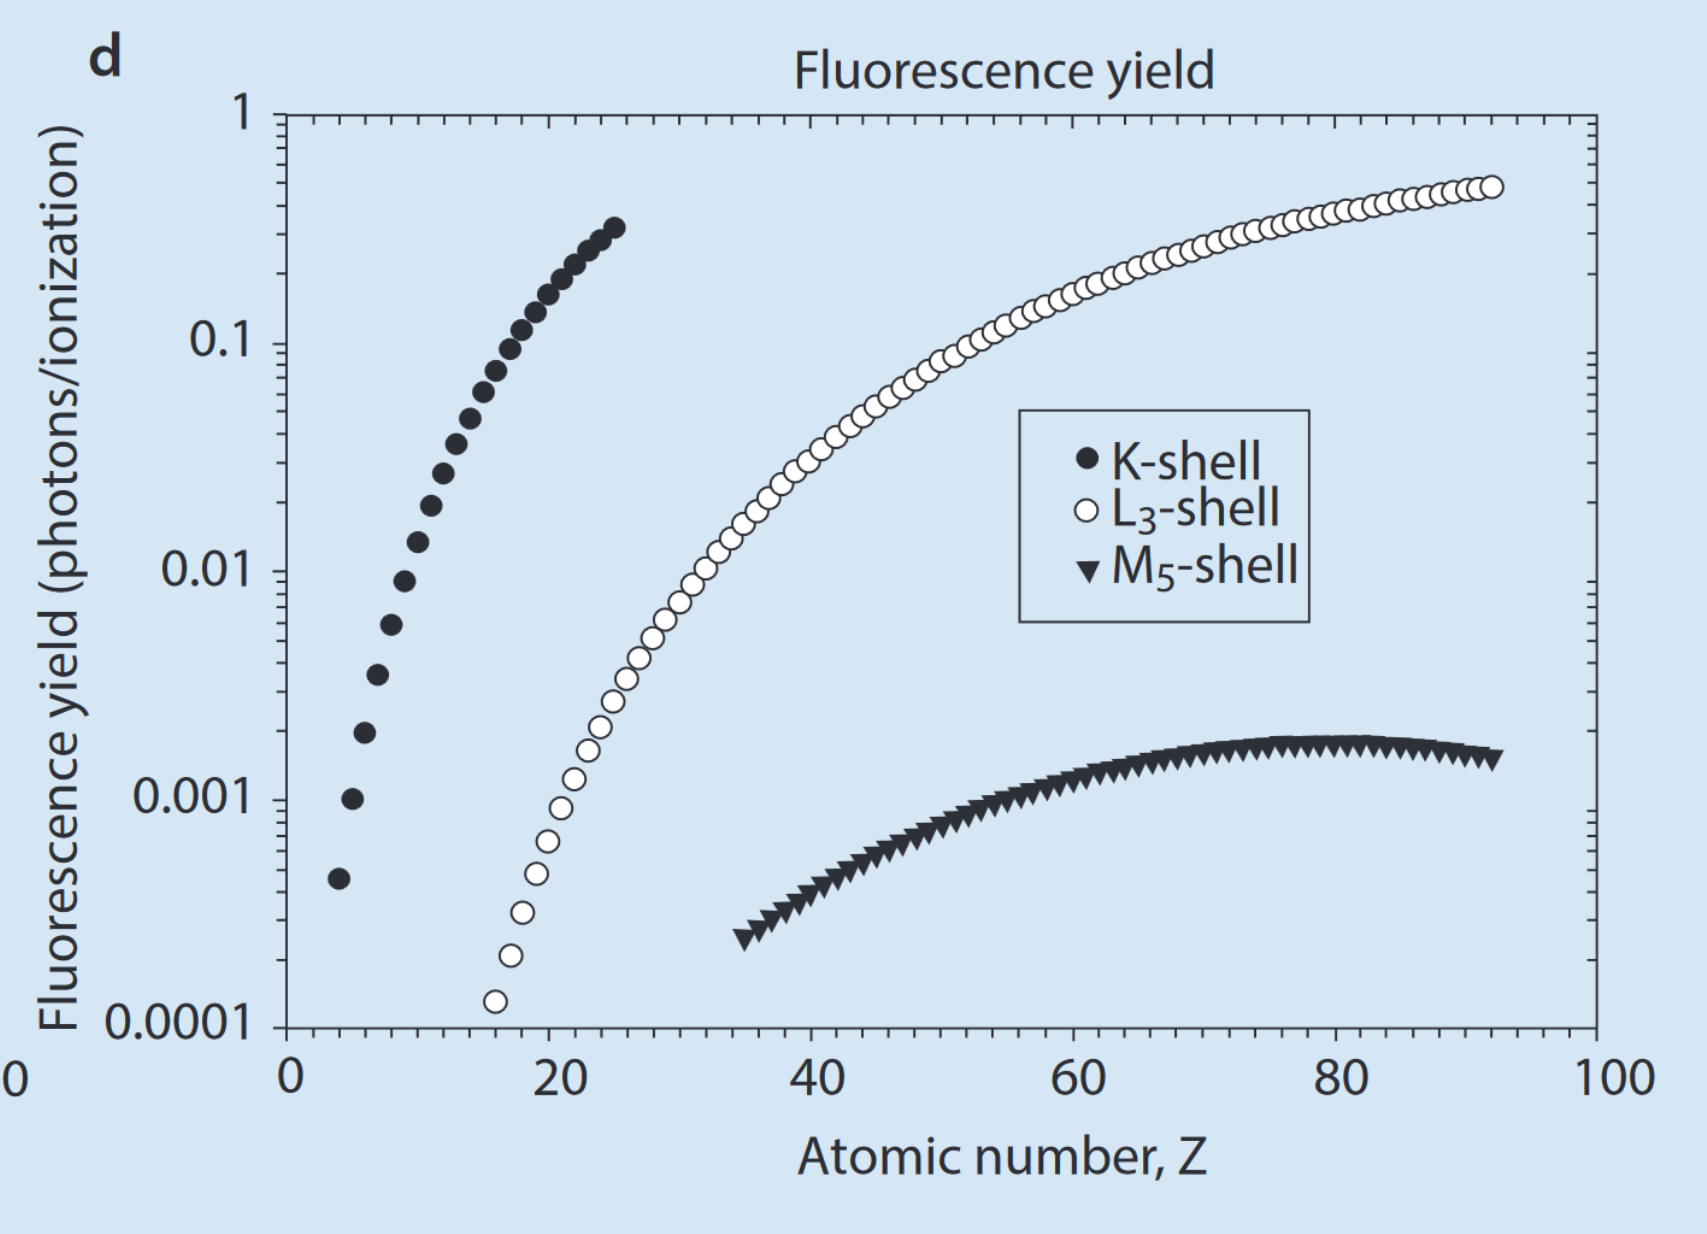
\includegraphics[width=0.7\textwidth]{figures/fluorescence_yield_Goldstein_Fig4-3-d.png}
    \caption{
        Fluorescent yield for K-, L- and M-shell, as a function of atomic number $Z$.
        The figure is copied from Goldstein \cite[Fig. 4.3 (d)]{goldstein_scanning_2018}.
    }
    \label{fig:theory:fluorescence_yield}
\end{figure}



\begin{equation}
    \label{eq:empirical:fluorescentyieldapprox}
    \omega = \frac{Z^4}{a + Z^4}
\end{equation}

% critical ionization energy
The critical ionization energy, $E_\textnormal{C}$, is the energy the incident beam need to ionize a core electron in an atom.
If the energy of the incident beam is lower than $E_\textnormal{C}$, the core electron is not ionized and no peak can be detected.
The critical ionization energy is dependent on the atomic number, $Z$, of the atom.
Higher $Z$ means higher $E_\textnormal{C}$, because the core electrons are bound stronger to the nucleus.
When the incident beam has an energy higher than $E_\textnormal{C}$ and continues to increase, the amount of ionization is not constant and not linear.
The amount of ionization with varying energy above $E_\textnormal{C}$ is dependent on the ionization cross section and the overvoltage, which again are dependent on what shell the ionization happens in.
The solution to this is empirically estimations and using k-factors where all factors like this is either cancelled out or included in the k-factor correction.

% Ionization cross section and overvoltage
% \ton{Is this good enough? If not, what do I write about the ionization cross section and overvoltage? What Mari wrote is for thin samples, I think. Why include it if I'm not going to use any equations about the ionization cross section or overvoltage? You said something about just write that intensity it is lower for low energy because of many reasons (absorption, efficiency), with the same reason that background is lower for low energy. But I kinda need to explain some reasons to use them in the discussion. Another question: in the k-factor all these other factors fall out, so EDS-people does not use these equations. Am I wrong?}

% TODO with comment from Ton:
% Cross sections are at the heart of explaining interactions and tabulate behaviour for different elements.
% You make a good point regarding thin samples, but that is a simplification. Mari used it to limit calculatiuons. If thick, need ZAF corrections (based on many models and assumptions, running a loop until converged). Aztek is not clear on this in default mode, and then the results becomes unsure. HyperSpy use thin film, but let you analyse spectra from bulk. The user must understand the background and the limitations. In this theory part, you address aspects that can possible play a part.
% In discussion can address what aspects can be better in the analysis, nothing that there are many. For future work, can say limit to thin or develop open-source for bulk.?

% Maybe the DTSA-II gives some hints what matters, see Goldstein or file:///C:/Users/helvoort/Downloads/getting-started-with-nist-dtsa-ii.pdf








% empirical weights in HyperSpy
HyperSpy have an integrated list of the characteristic X-rays, with both the energy and the weight of the lines.
% \brynjar{I guess the weights are empirically estimated, but I have not found any information about how they are estimated. In addition: I'm not sure if HyperSpy adjust the line height to the spectrum, or if it knows that Ga K$\alpha$ are higher than As K$\alpha$ as in \cref{fig:theory:GaAs30keV-8-12-keV}.}
Goldstein uses different intensity weights for isolated atoms, thin foils and bulk samples \cite[Ch. 4.2.6]{goldstein_scanning_2018}, and all are dependent on the atomic number and ionized shell.
One could venture down the rabbit hole of finding the theoretical weights for different lines, but that will not be done in this thesis.














\section{Data processing}
\label{sec:theory:data}

This section on data processing covers what HyperSpy is, quantification with Cliff-Lorimer and calibration of a spectrum.






\subsection{HyperSpy}
\label{sec:theory:data:hyperspy}


HyperSpy is a Python package for processing and analyzing signals and multidimensional data.
It is open-source and free to use, and is developed by a community of scientists and engineers.
Updates and discussion about the package is done on GitHub at \url{https://github.com/hyperspy/hyperspy}.
The documentation for the package is available at \url{https://hyperspy.org/hyperspy-doc/current/index.html}.
The origin of HyperSpy is in the field of TEM, but it has been expanded to include other fields such as SEM.

Currently, HyperSpy have implemented functions for quantification of TEM EDS data, but not for SEM EDS data.
The functions and methods for treating SEM EDS data is still limited, while the methods for TEM EDS data is more developed.








%
% 
% k-factors
% k-ratios
\subsection{Cliff-Lorimer and the k-factors}
\label{sec:theory:empirical:kfactors}

One of the included quantification methods in HyperSpy is Cliff-Lorimer \cite{CL1975}.
The method is based on the thin-foil criteria, where it is assumed that all absorption and fluorescence can be ignored.
The CL method is based on the assumption that the intensity of the characteristic X-rays from two elements in the sample is proportional to the concentration of the elements.
Each element has a correction factor for the intensity emitted from its lines, which is called the k-factor.
The concentrations, intensities and k-factors are related by the following equation:

\begin{equation}
    \frac{C_\textnormal{a}}{C_\textnormal{b}} = \frac{k_\textnormal{a} I_\textnormal{a}}{k_\textnormal{b} I_\textnormal{b}} = k_\textnormal{ab}  \frac{I_\textnormal{a}}{I_\textnormal{b}}
\end{equation}

If the same method is to be applied for a sample where the thin-foil criteria is not valid, a correction matrix must be applied.
The correction matrix in SEM EDS is correcting for the atomic number effects (Z), the absorption in the bulk sample (A) and the fluorescence (F).
This is called the ZAF correction matrix \cite{ZAF_1978}.

%
% calibration of the spectrum
\subsection{Calibration of the spectrum}
\label{sec:theory:calibration}

% General calibration, which needs peak centers. Just mention fitting.
% my notebook
% equation dispersion = e2 - e1 / c2 - c1

Calibration of a spectrum is finding the energy per channel of the spectrum and the zero-offset.
The calibration process is a general process, and is not specific to SEM EDS.
In EDS the calibration can be calculated with two known peaks.
$E_1$ and $E_2$ is the energy of the two characteristic X-rays, and $c_1$ and $c_2$ is the channel number of the two characteristic X-rays.

\begin{equation}
    \label{eq:theory:calibration:dispersion}
    \textnormal{Dispersion} = \frac{E_2 - E_1}{C_2 - C_1}
\end{equation}

With the dispersion, the zero-offset can be calculated with the following equation

\begin{equation}
    \label{eq:theory:calibration:offset}
    \textnormal{Zero-offset in channels} = C_1 - E_1 \cdot \textnormal{Dispersion}
\end{equation}














\section{Detection system}
\label{sec:theory:detectionsystem}

This section covers briefly the EDS detector.
It is expected that the reader knows the working principles of a SEM.


\subsection{EDS detector}
\label{sec:theory:edsdetector}

An EDS system consist of a detector inside an electron microscope and a computer controlling the system.
The detector is a silicon drift detector (SDD) that is sensitive to X-rays.
The incident electron beam hits the sample where X-rays are generated and emitted.
When the X-rays hit the detector, the electrons in the silicon drift detector are excited and the electrons drift to the anode.
This is registered as a signal, and the amount of electrons is proportional to the intensity of the X-rays.
When a signal is being registered, the detector cannot receive any more signals, and this is called the dead time.
The computer controls the detector and shuts the detector off and on during the acquisition of the spectrum.
Even though it looks like a spectrum is acquired simultaneously for all the energies in the spectrum, the detector can only register one photon at a time.
The registered photons are registered in channels, which are a small energy range.

The EDS system is described nicely in Skomedal \cite{skomedal_improving_2022}, and more in detail in Goldstein \cite{goldstein_scanning_2018}.
A nice table with relevant parameters for the EDS system is found in "Getting Started with NIST* DTSA-II" by Ritchie \cite{NIST-DTSA-II}.

% Ton:
% here are several things to write out
% file:///C:/Users/helvoort/Downloads/getting-started-with-nist-dtsa-ii.pdf
% has also some comments on detector calibration, I believe Goldstein as well.

%   - the detection system
%     - detector efficiency
%     - detector resolution
%     - dead time
%     - angle/placement of detector
%     - beam issues
%     - stray: secondary excitations in the sample
%     - Si stray
%     - holder / chamber stray detection





% Data processing (hvis jeg kommer dit)
% - ML, støybehandling
% - future work?
% - Ton er skeptisk



% PCA, ICA ???????? Gjøre noe faktisk statistikk?

